\documentclass{beamer}
\usetheme{dianahep}

%
% Title definitions
%

\title{Software Upgrade for HL-LHC}
\author{Peter Elmer - Princeton University}
\date{9 September, 2016 \\ RDMS CMS Collaboration Meeting}

\begin{document}
\maketitle
%\insertframenumber/\inserttotalframenumber

%
% Presentation body
%

\setbeamertemplate{footline}[frame number]

\begin{frame}
\frametitle{A Software ``Upgrade'' for the HL-LHC?}

Looking forward to the next 10 years, we see a number of challenges for software and computing:

\begin{itemize}
\item {\bf Scale:} The HL-LHC will provide 100 times the current data, with significantly increased data (pileup) and detector complexity.
\item {\bf Peformance/cost:} Estimates of computing needs run faster than Moore's Law by factors of 3-30
\item {\bf Technology/Market evolution:} the return of heterogeneity; technology change will also make it challenging to exploit Moore's Law without software evolution.
\item {\bf Sustaintability:} Most of the current software, which defines our capabilities, was designed 15-20 years ago: there are many software sustainability challenges.
\end{itemize}

\end{frame}



\begin{frame}
\frametitle{Why Software? Software is {\em the} Cyberinfrastructure}

\begin{figure}[htbp]
\begin{center}
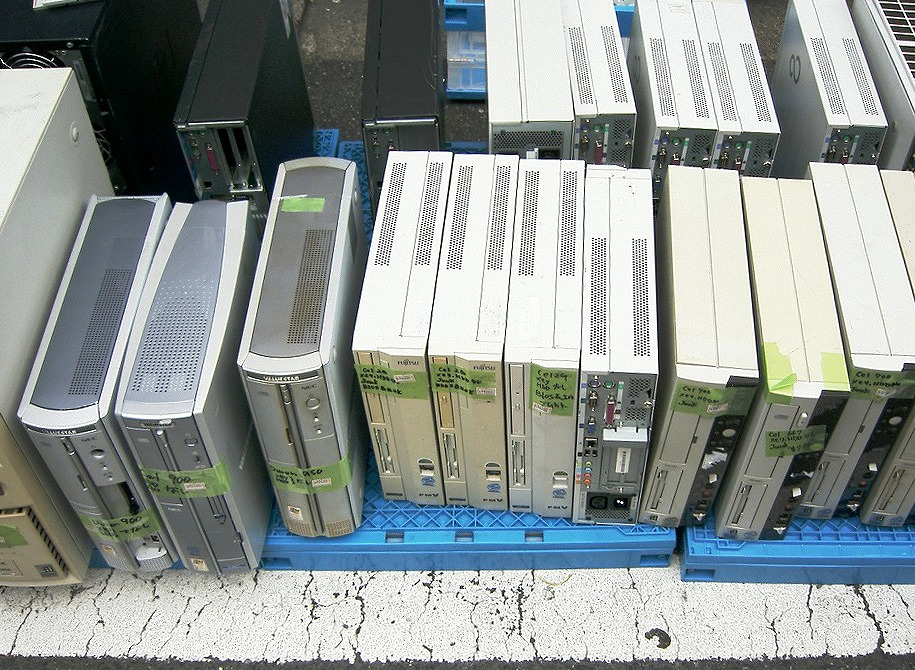
\includegraphics[width=0.7\textwidth]{images/Junk_desktop_personal_computer.jpg}
%\caption{}
%\label{fig:example2}
\end{center}
\end{figure}

\begin{center}
\small{Computer hardware is a consumable. \\ What we keep, and invest in, over 
time is the software.}
\end{center}

\end{frame}



\begin{frame}
\frametitle{HEP Software Ecosystem}

\begin{figure}[htbp]
\begin{center}
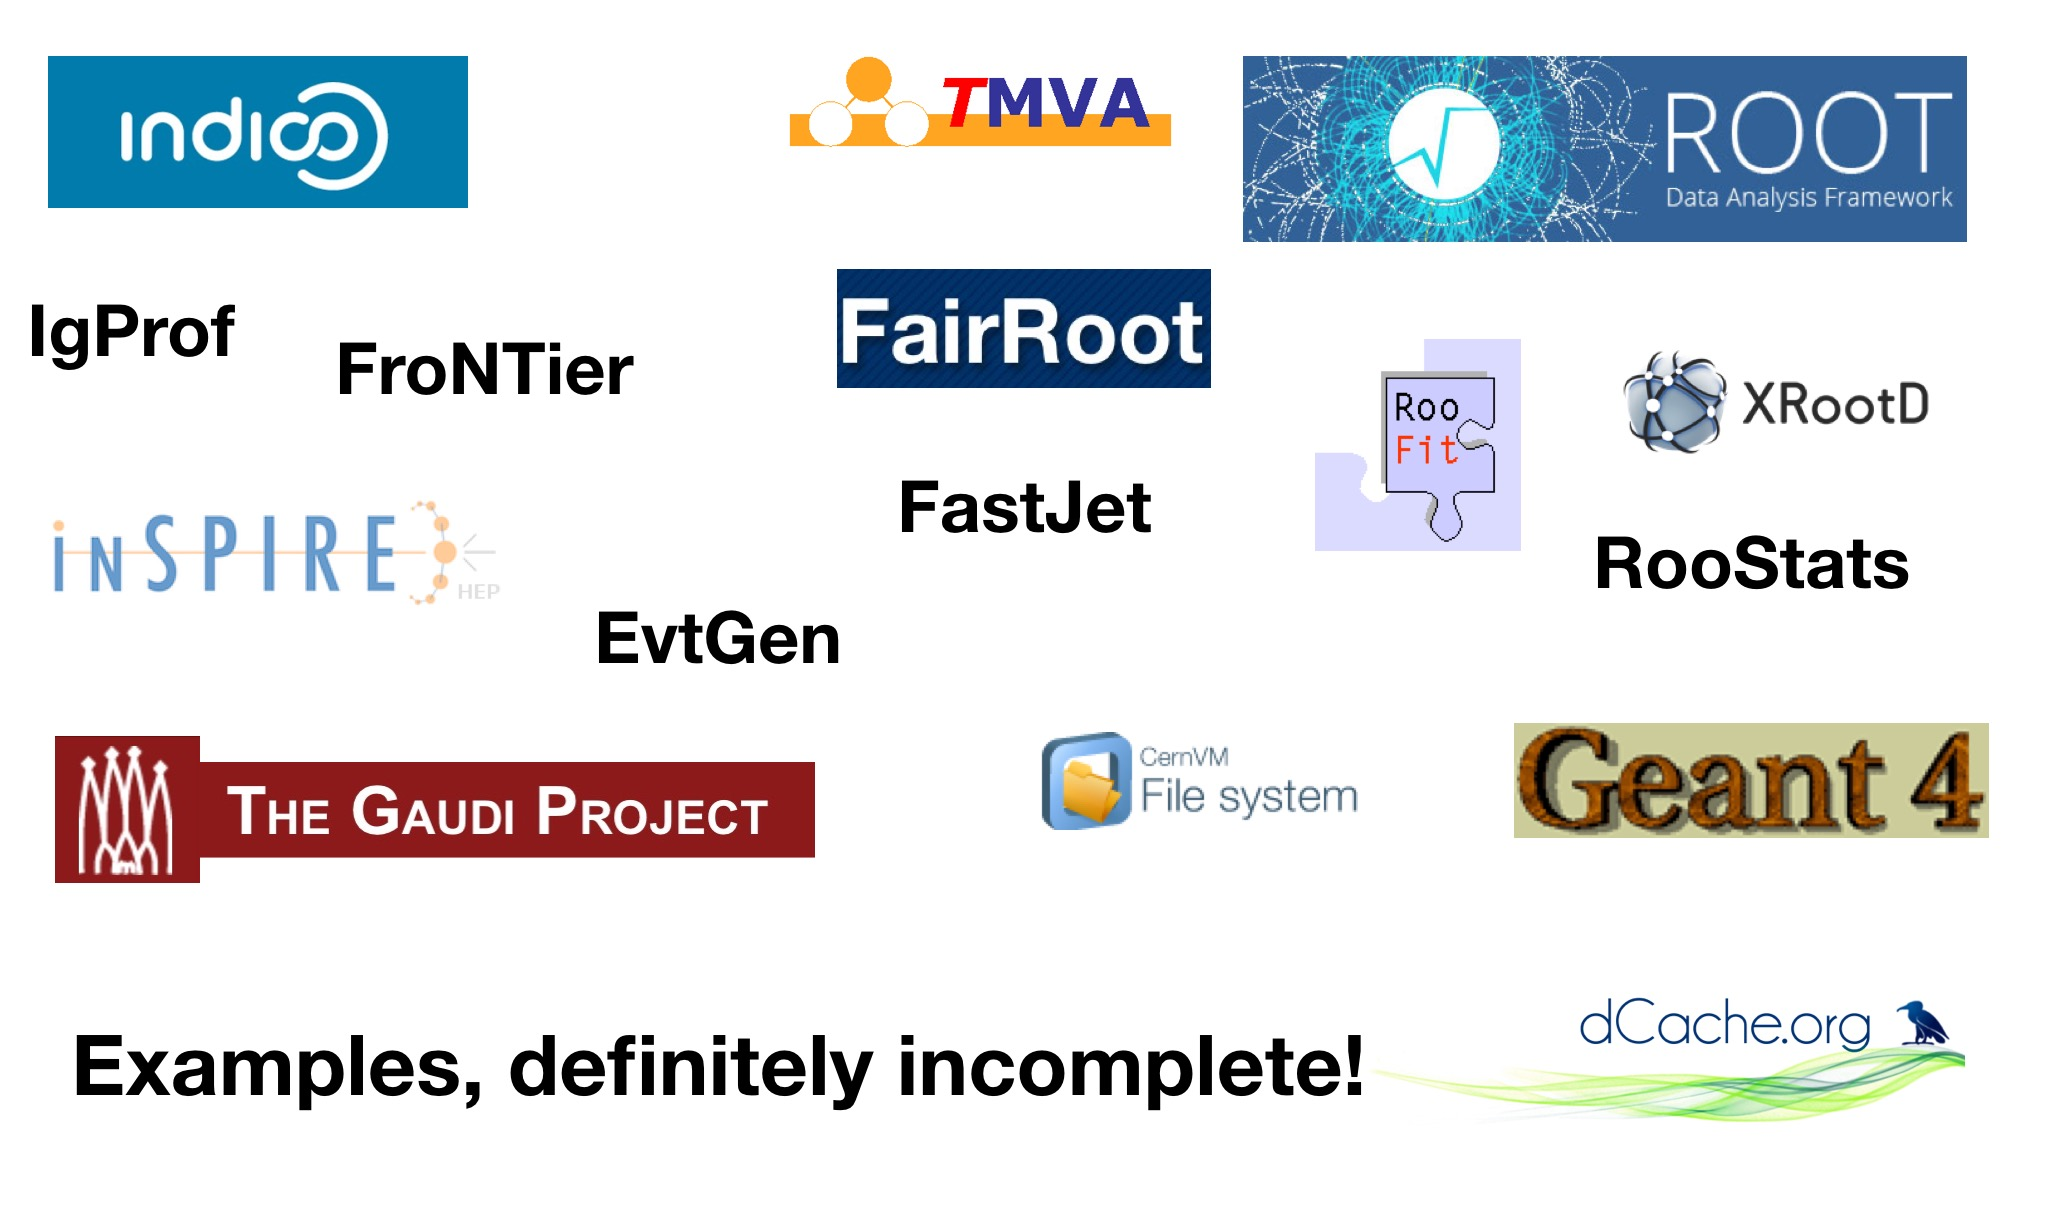
\includegraphics[width=0.9\textwidth]{images/hep-software-ecosystem.jpg}
\end{center}
\end{figure}

\end{frame}



\begin{frame}
\frametitle{Software and Computing for the HL-LHC Era - Scale}

The DOE and NSF jointly invest $ \approx \$ 35 $M/year in
ATLAS and CMS software and computing, about half in hardware plus operations,
about half in software professionals.
The LHC funding agencies, worldwide, invest about $ \$ 150 $M/year
in these enterprises.
In 2014, the LHC experiments used almost 175 PB of tape storage and
slightly more disk storage.
The event rate anticipated for the HL-LHC era is 100 times greater,
and even assuming the experiments significantly reduce the
amount of data stored per event,
the total size of the datasets will be well into the exabyte
scale;
they will be constrained primarily by costs and funding levels,
not by scientific interest.
One long-term goal of a software upgrade for HL-LHC
will be
maximizing the return-on-investment to enable break-through
scientific discoveries using the  HL-LHC detectors.


\end{frame}



\begin{frame}
\frametitle{Processor evolution - Power dissipation vs Time}

\begin{figure}[htbp]
\begin{center}
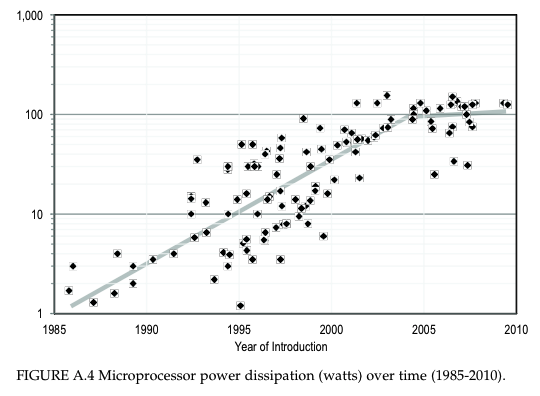
\includegraphics[width=0.75\textwidth]{images/moore1.png}
\end{center}
\end{figure}

\small{Power density limitations in processors fundamentally changed the game from about 2005.}

\end{frame}



\begin{frame}
\frametitle{Processor evolution - Clock Frequency vs Time}

\begin{figure}[htbp]
\begin{center}
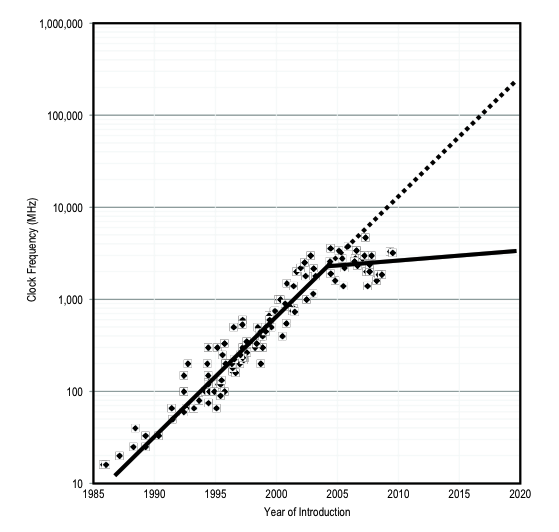
\includegraphics[width=0.5\textwidth]{images/moore2.png}
\end{center}
\end{figure}

\small{Single core performance stalled, leading to multi/manycore, specialization, need for parallelization of algorithms and design for performance.}

\end{frame}



\begin{frame}
\frametitle{Back to heterogeneous systems?}

Building the worldwide distributed LHC computing grid was largely made possible by the convergence on Linux on (commodity) Intel x86 processors around the year 2000. Building the WLCG at this scale in the heterogeneous workstation era would have been quite difficult. For better or for worse, heterogeneity is returning:

\begin{itemize}
\item Diversity of computing processor architectures (general purpose cores vs specialized processors)
\item Owned vs commercial/cloud providers
\item Some pressure to use systems traditionally designed for other types of applications (e.g.\ HPC/supercomputer as opposed to HTC/high-throughput systems)
\item Possible further commoditizing market pressures (e.g. mobile)
\end{itemize}

\end{frame}



\begin{frame}
\frametitle{What is software sustainability?} 
\begin{itemize}
\item {\bf Dependent Infrastructure:} Will the infrastructure element continue to provide the same functionality in the future, even when the other parts of the infrastructure on which the element relies change?
\item {\bf Collaborative Infrastructure} Can the element be combined with other elements to meet user needs, as both the collaborative elements and the individual elements change?
\item {\bf New Users:} Is the functionality and usability of the infrastructure element clearly explained to new users? Do users have a mechanism to ask questions and to learn about the element?
\item {\bf Existing Users:} Does the infrastructure element provide the functionality that current users want? Is it modular and adaptable so that it can meet the future needs of the users?
\item {\bf Science:} Does it incorporate and implement new science and theory as they develop?
\end{itemize}

\tiny{ Katz, D.S. \& Proctor, D., (2014). A Framework for Discussing e-Research Infrastructure Sustainability. Journal of Open Research Software. 2(1), p.e13. DOI: http://doi.org/10.5334/jors.av}
\end{frame}



\begin{frame}
\frametitle{Likely constraints to fund a ``Software Upgrade''}

It appears unlikely that significant increases in investments in software 
will be made by funding agencies purely from particle physics budgets 
and/or into individual experiments. Other opportunities do perhaps exist,
but often imply constraints, for example:

\begin{itemize}
\item Investments into software impacting multiple experiments 
\item Investments into development with impact beyond particle physics 
\item Investments into development permitting use of computing facilities (e.g. HPC) planned for other non-HEP purposes
\item Investments requiring collaborations with Computer Science or Industry
\end{itemize}

Building the LHC software in use today was possible without too many such constraints. The good news is that the community (with an existing LHC computing system) is better positioned today to make effective progress even with such constraints.

\end{frame}


\begin{frame}
 \frametitle{HSF As Umbrella For HEP Community Activities}
The HEP Software Foundation (HSF) (http://hepsoftwarefoundation.org) was created 1.5 years ago as a means for organizing our community to address the software challenges of future projects like the HL-HLC.
An initial set of collaborative activities have begun (see recent HSF workshop 
at LAL-Orsay). The HSF has the following objectives:

\begin{itemize}
\item Catalyze new common projects
\item Promote commonality and collaboration in new developments to make the most of limited resources
\item Provide a framework for attracting effort and support to S\&C common projects (new resources!)
\item Provide a structure to set priorities and goals for the work
\end{itemize}


\end{frame}




\begin{frame}
\frametitle{Community Roadmap for HEP S\&C}

\noindent As a step towards software upgrades for HL-LHC, the WLCG has charged the HSF and the experiments to prepare a {\bf Community White Paper for HEP Software and Computing (CWP)}.  This community white paper should describe a global
vision and roadmap for software and computing for the HL-LHC era and HEP in the 2020s;
it should include discussions of elements that are common to
the HEP community (LHC community, etc.) as a whole and those that are specific
to the individual experiments. It should also discuss the relationship of the 
common elements to the broader scientific computing communities.
\vskip 0.15in
This document will be a concrete step in the HL-LHC process over the next years and can play a role in discussing possible funding scenaries for a ``software upgrade''.

\end{frame}



\begin{frame}
\frametitle{Community White Paper (CWP) - Outline}

\begin{itemize}
  \item
    a broad overview of the grand challenge science (HL-LHC, HEP);
  \item
    how new approaches to computing and software can enable and
    radically extend the physics reach of the detectors;
  \item
    what computing and software research will be required so that
    (for example) computing and software Technical Design Reports
    can be prepared several years before Run 4 of the LHC begins;
    this will include studies of hardware and software architectures
    and life-cycle processes and costs.
   \item
    identify specific software elements and frameworks that will
    be required for the HL-LHC era which can be built and tested
    during Run 3.
   \item
     organizational issues for the common software and for
     coordinating research of common interest, even when the
     final products will be specific to individual experiments.
  \item
     software development and documentation tools for
     writing sustainable software;
%  \item identifying and mitigating potential risks
\end{itemize}


\end{frame}



%\begin{frame}
\frametitle{Derived Plans and Proposals} 
The CWP should be the document from which specific plans/proposals can be derived. The US NSF, for example, has indicated a possible path forward to real resources (next slide) to fund a part of such an upgrade project. In parallel to the CWP process proposed here we will prepare a ``Strategic Plan'' for the NSF.
\vskip 0.15in
It should also provide a better context for engaging computer scientists, other sciences and industry (e.g. through CERN Openlab)
\vskip 0.15in
As a community we should be pursuing and preparing the ground for these opportunities in parallel to the preparation of the CWP.
\end{frame}




\begin{frame}
\frametitle{Detector Simulation, Triggering, Event Reconstruction and Visualization} 
\scriptsize{
Challenges surrounding high pile-up simulation,
including the CPU resources needed for large statistics samples
needed to compare with data from high trigger rates, high memory
utilization, generation and handling of the large (min-bias) samples
needed to achieve accurate description of high pile-up collision
events, and a flexible simulation strategy capable of a broad
spectrum of precision in the detector response, from ``fast''
(e.g. parametric) simulation optimized for speed to full simulation
in support of precision measurements and new physics searches
(e.g. in subtle effects on event kinematics due to the presence of
virtual particles at high scale).
Software required to emulate upgraded detectors (including the
trigger system) and support determination of their optimal
configuration and calibration.
Software in support of triggering
during the HL-LHC, including algorithms for the High-level Trigger,
online tracking using GPUs and/or FPGAs, trigger steering, event
building, data ``parking'' (for offline trigger decision), and data
flow control systems. New approaches to event reconstruction, in
which the processing time depends sensitively on instantaneous
luminosity, including advanced algorithms, vectorization, and
execution concurrency and frameworks that exploit many-core
architectures. In particular, charged particle tracking is expected
to dominate the event processing time under high pile-up
conditions. Visualization tools, not only in support of upgrade
detector configurations and event displays, but also as a research
tool for data analysis, education, and outreach using modern tools
and technologies for 3D rendering, data and geometry description and
cloud environments.
}
\end{frame}



\begin{frame}
\frametitle{Data Access and Management, Workflow and
Resource Management}
\scriptsize{ 
Data handling systems that scale to the Exabyte level during the
HL-LHC era and satisfy the needs of physicists in terms of metadata
and data access, distribution, and replication. Increasing
availability of very high speed networks removes the need for CPU
and data co-location and allows for more extensive use of data
access over the wide-area network (WAN), providing failover
capabilities, global data namespaces, and caching. Event-based data
streaming as complementary to the more traditional dataset-based or
file-based data access, which is particularly important for
utilizing opportunistic cycles on HPCs, cloud resources, and campus
clusters where job eviction is frequent and stochastic. Workflow
management systems capable of handling millions of jobs running on a
large number of heterogeneous, distributed computing resources, with
capabilities including whole-node scheduling, checkpointing, job
rebrokering, and volunteer computing. Systems for measurement and
monitoring of the networking bandwidth and latency between resource
targets and the use of this information in job
brokering. Software-defined networking technologies which enable
networks to be configurable and schedulable resources for use in the
movement of data.
}

\end{frame}



\begin{frame}
\frametitle{ Physics generators, Data Analysis and Interpretation, Data and Software Preservation}
\scriptsize{ 
There are many theory challenges in the HL-LHC era, among them are
improving the precision of SM calculations, better estimation of
systematic uncertainties, and elucidation of promising new physics
signals for the experiments. Software needed to make connection
between observations and theory include matrix element generators,
calculation of higher-order QCD corrections, electroweak
corrections, parton shower modeling, parton matching schemes, and
soft gluon resummation methods. Physics generators that employ
concurrency and exploit many-core architectures will play an
important role in HL-LHC, as well better sharing of code and
processing between LHC experimenters and phenomenologists. Data
analysis frameworks that include parallelization, optimized event
I/O, data caching, and WAN-based data access. Analysis software
that employs advanced algorithms and efficiently utilizes many-core
architectures. Tools and technologies for preservation and reuse of
data and software, preservation and re-interpretation of physics
results, analysis providence and workflow ontologies, analysis
capture, and application packaging for platform abstraction. Future
software repositories and build platforms that leverage advances in
these areas and improved software modularity and quality control
that will allow a broader community of people to effectively
contribute to software in the HL-LHC era.}

\end{frame}



\begin{frame}
\frametitle{Working groups - example questions to address}

In addition to addressing issues specific to a given topic,
each group should presumably address questions which cut across boundaries,
including:
\begin{itemize}
\item
  What are the specific challenges for the HL-LHC (IF, etc.)?
\item
  What opportunities exist to exploit new or advanced
  algorithms (e.g.\ deep learning)?
\item
  How can emerging architectures improve the bang-per-buck and what
  software evolution is needed to exploit them?
\item
  Which problems are specific to individual experiments and which
  are common to (for example) the HL-LHC experiments or to HEP
  and nuclear physics experiments
  more generally?
\item
  What is required to make common software packages sustainable?
\end{itemize}


\end{frame}



\begin{frame}
\frametitle{Status}

\noindent 
The proposal for a general Community Roadmap has been widely discussed with all of the LHC experiments and the HEP Software Foundation (HSF). There is broad support for the idea. \\
\vskip 0.1in
The CWP roadmap plan, to be carried out by HSF, was presented to the LHCC. It fits with the current notion of HL-LHC computing TDRs in $\sim$2019.\\
\vskip 0.1in
WLCG has produced a charge for this CWP to the HSF and the LHC experiments (see separate link) with an aim to complete it by the end of August, 2017. \\
\vskip 0.1in
The HSF is beginning the process of organizing working groups and planning for 
some dedicated workshops. We will also use sessions at existing meetings when possible. \\

\end{frame}




\begin{frame}
\frametitle{Community Roadmap Process}

We propose a series of workshops over the next year to build the community roadmap:

\begin{itemize}
\item Organization of working groups with experiments by September.
\item A half-day ``pre-CWP'' (Sun 9 Oct) just before CHEP in San Francisco
\item A ``kick-off'' workshop at UC San Diego in Jan2017
\item Several dedicated ``topical'' workshops between Jan-Jun 2017 covering software required in the various areas:
\begin{itemize}
\item Detector Simulation, Triggering, Event Reconstruction and Visualization
\item Data Access and Management, Workflow and Resource Management
\item Physics generators, Data Analysis and Interpretation, Data and Software Preservation
\end{itemize}
\item A final workshop in summer 2017 (near CERN?)
\end{itemize}

We will build on existing community activities when possible (e.g.\ DPHEP, Reco Algorithms Forum/CTD, IML). 

\end{frame}



\begin{frame}
 \frametitle{What should the community roadmap process accomplish?}
Going back to the subset of HSF goals I listed earlier:

\begin{itemize}
\item Catalyze new common projects
\item Promote commonality and collaboration in new developments to make the most of limited resources
\item Provide a framework for attracting effort and support to S\&C common projects (new resources!)
\item Provide a structure to set priorities and goals for the work
\end{itemize}

The workshop process, the community roadmap white paper and (simultaneously) the pursuit of specific plans/proposals will support precisely these goals.

\end{frame}




\begin{frame}
\frametitle{Possible routes to a ``Software Upgrade''}

\begin{itemize}
\item If we are aiming at a larger ``software upgrade'' project towards the HL-LHC, an additional ingredient is to find (or liberate/reallocate) the resources to realize this roadmap. 
\item We need both initial exploratory R\&D and eventual development projects!
\item In the US, both the NSF and the DOE have at least the notion of eventual resources and/or organization for new common projects in HEP (NSF: SI2, DOE: HEP CCE)
  \begin{itemize}
   \item The US NSF has funded a ``conceptualization'' (planning) project with a possible path towards a ``Software Institute''.
   \item The US DOE has seeded the ``Center for Computing Excellence'' with some initial resources. 
  \end{itemize}
\item We hope that a clear community roadmap will bring these and other partners together for an HL-LHC software upgrade.
\end{itemize}

\end{frame}




\begin{frame}
\frametitle{Software Infrastructure for Sustained Innovation (SI2)}

\begin{figure}[htbp]
\begin{center}
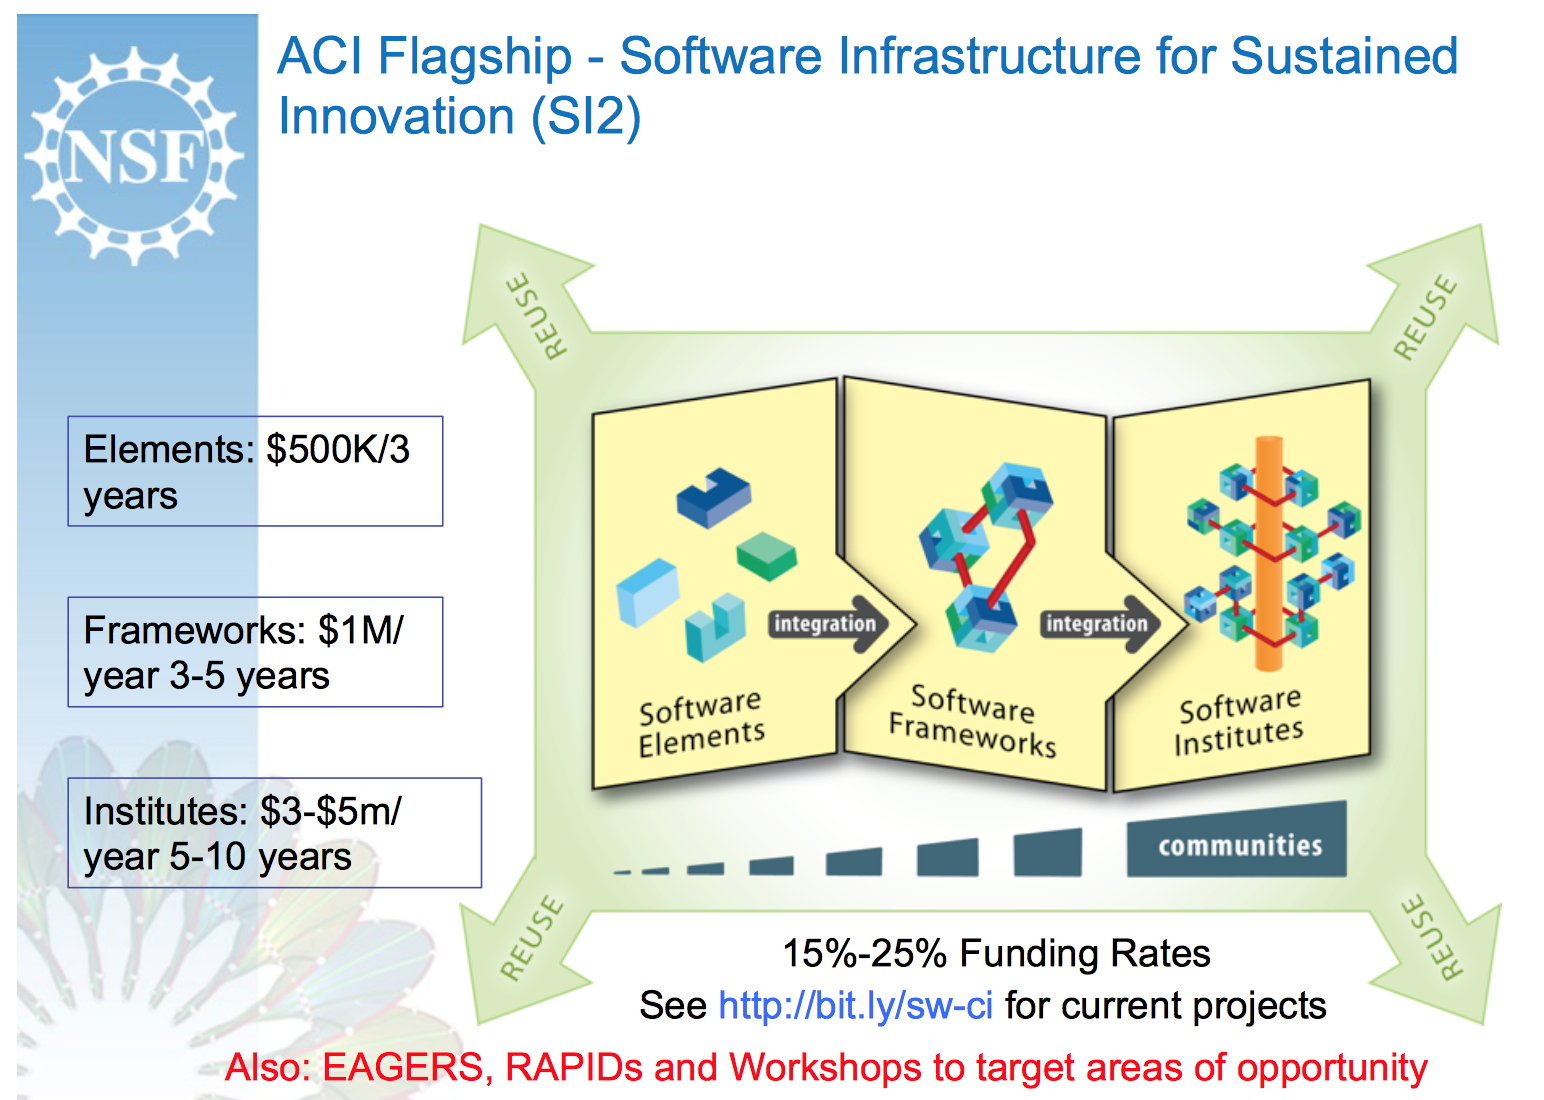
\includegraphics[width=0.75\textwidth]{images/ramnath-si2-pi-meeting-2016.png}
%\caption{}
\label{fig:nsfsi2}
\end{center}
\end{figure}

DIANA-HEP is a ``Software Framework'' (SSI).  The ``Software Institute'' (S2I2) class of award could provide some resources for software upgrades.

\end{frame}



\begin{frame}
\frametitle{DOE HEP-CCE}


\begin{figure}[htbp]
\begin{center}
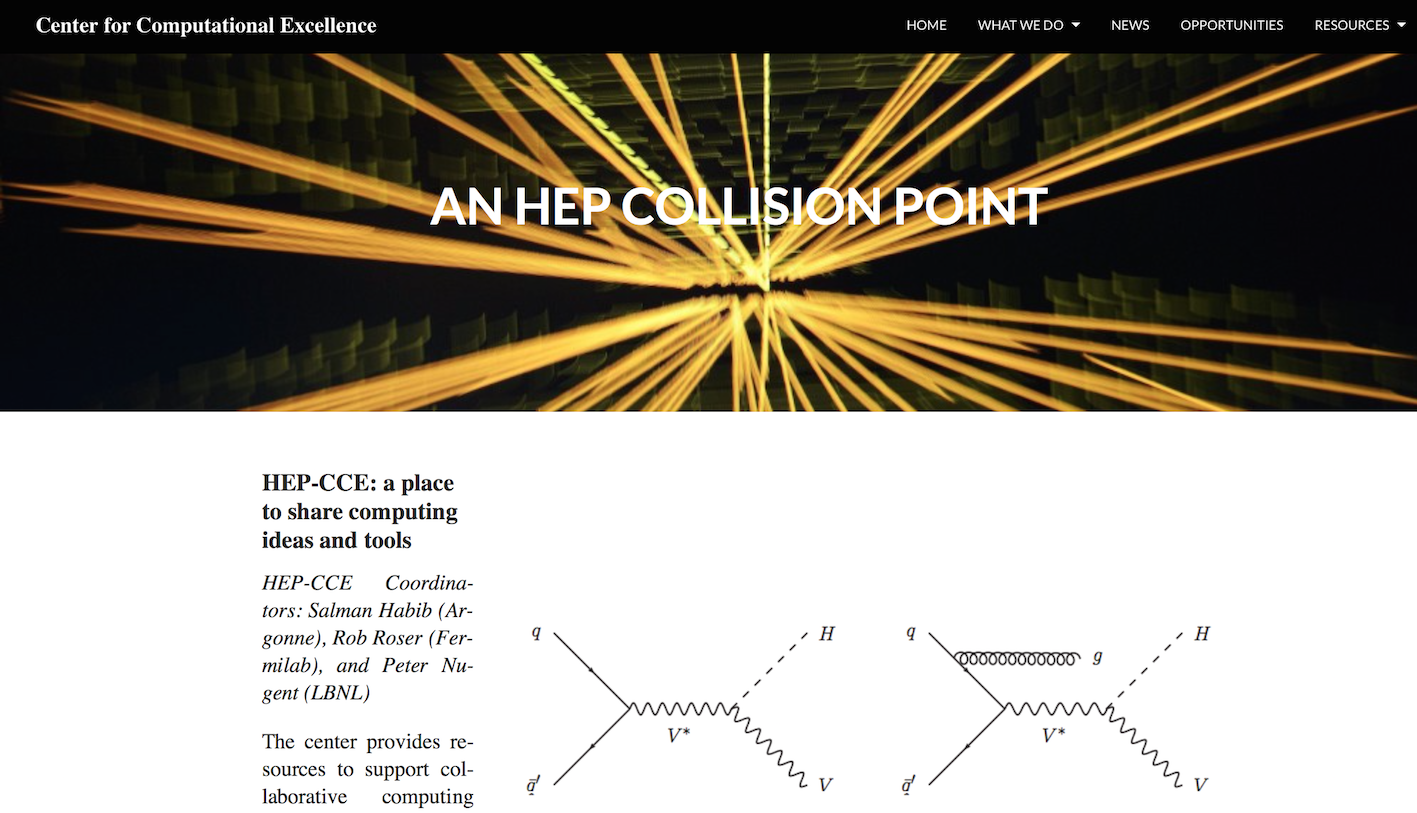
\includegraphics[width=0.7\textwidth]{images/hepcce-webpage.png}
\end{center}
\end{figure}

\small{Project in formative stage, small initial projects and particular interests in exploiting HPC/supercomputer resources.}

\end{frame}



%\begin{frame}
\frametitle{DOE HEP-CCE}

 Contents of the first slide

\end{frame}



%\begin{frame}
\frametitle{NSF SI2-S2I2 Software Institute}

NSF SI2-S2I2 includes two subclasses of awards (two steps!):
\begin{itemize}
\item \underline{Conceptualization Awards} - which are planning awards aimed at organizing an interdisciplinary community and understanding their software requirements and challenges (\$500k, 1-2 years)
\item \underline{Implementation Awards} - which will be made to implement community activities that support software infrastructure, for example, such as those developed by the conceptualization awards (\$3-5M/year, 5 years)
\item The first solicitation for implementation proposals was last June; we anticipate announcements of these awards shortly.
%\item \url{http://www.nsf.gov/pubs/2015/nsf15553/nsf15553.htm}
\end{itemize}

We submitted a conceptualization proposal to NSF last August (2015):
\begin{itemize}
\item Conceptualization of an $ S^2 I^2 $ Institute for High Energy Physics
\item \url{http://cern.ch/elmer/s2i2-2015-nsf-proposal.pdf}
\item Status: recommended for funding, awaiting awards
\end{itemize}

\end{frame}




\begin{frame}
\frametitle{Other R\&D and/or Code Modernization Projects}

\begin{itemize}
\item GeantV project (CERN, FNAL, Intel/CERN)
\item ROOT evolution (CERN/continuous, FNAL, Intel/Princeton, DIANA)
\item ``Big Data'' project (FNAL, CERN, Princeton, DIANA)
\item Multiple Cloud projects (incl. work with Amazon Web Services)
\item Efforts by CMS to work on NERSC HPC, Atlas to work on Argonne HPC
\item AIDA2020 Software work package (vectorized geometry, alignment, frameworks)
\item Significant grass roots interesting in Machine Learning 
\item Many other small efforts
\end{itemize}

\end{frame}



\begin{frame}
\frametitle{The DIANA/HEP project}

\begin{itemize}
\item Data Intensive ANAlysis for High Energy Physics (DIANA/HEP)
\item The primary goal of DIANA/HEP is to develop state-of-the-art tools for experiments which acquire, reduce, and analyze petabytes of data.
\item DIANA is not a piece of software itself, but a collaborative project to improve and extend analysis tools as sustainable infrastructure for the community.
\item Funded by NSF ``Software Infrastructure for Sustained Innovation'' (SI2) program
\item 4-year project, 6-7FTE total
\item Princeton, NYU, UCincinnati, U.Nebraska-Lincoln
\item The PIs are involved in Atlas, CMS and LHCb
\end{itemize}

\end{frame}



%\begin{frame}
\frametitle{The DIANA/HEP Project - Goals}

\begin{figure}[htbp]
\begin{center}
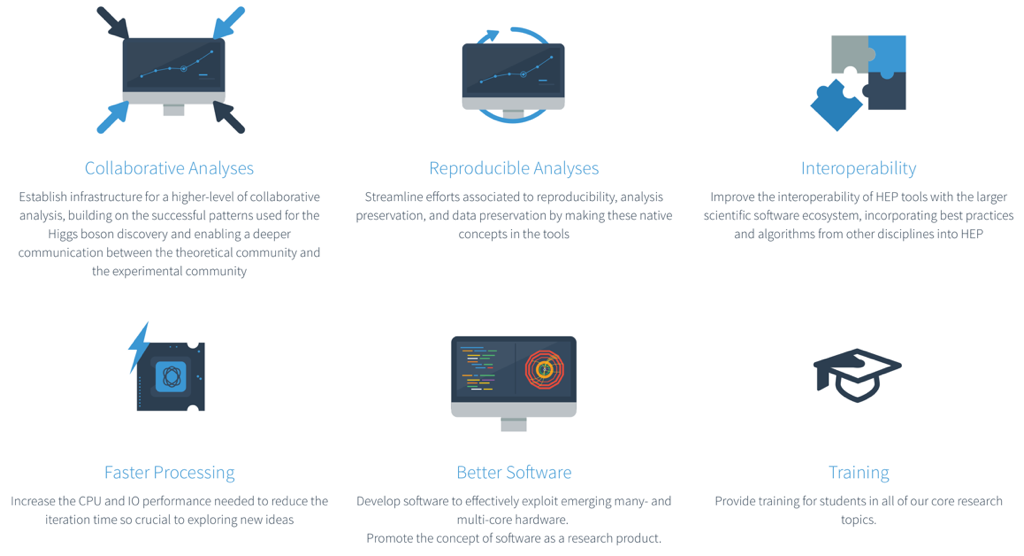
\includegraphics[width=1.0\textwidth]{images/20160610-diana-goals.png}
\end{center}
\end{figure}

\end{frame}



\begin{frame}
\frametitle{The DIANA/HEP Project (http://diana-hep.org)}

\begin{figure}[htbp]
\begin{center}
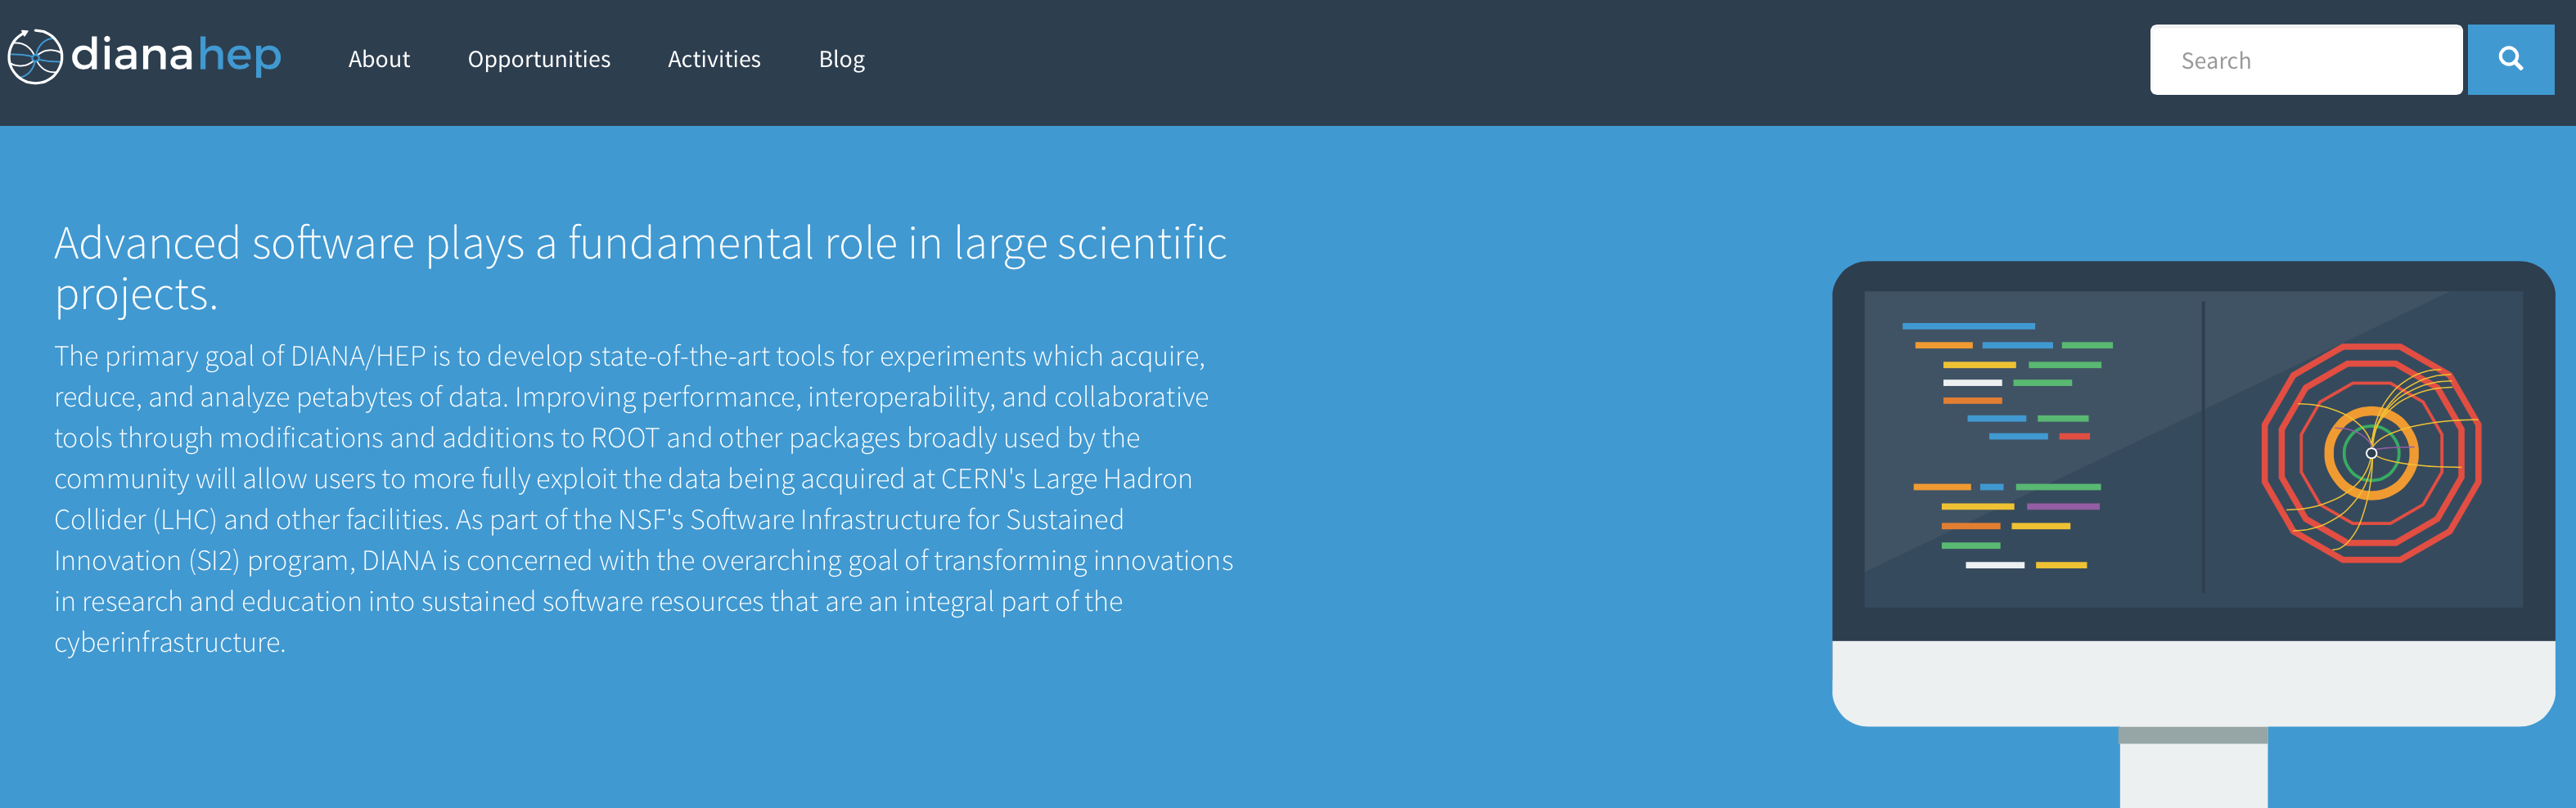
\includegraphics[width=1.0\textwidth]{images/20160610-diana-hep-banner.png}
\end{center}
\end{figure}

The project started (with personnel) in January 2016
\vskip 0.15in
Initial projects include: interoperability of HEP tools (ROOT) with Big Data tools such as Apache Spark and the scientific Python ecosystem, Development of machine learning research software and applications to HEP, I/O performance optimizations in ROOT

%\center{http://diana-hep.org}

\end{frame}



%\begin{frame}
\frametitle{Related NSF R\&D projects supporting HEP S\&C}

\begin{itemize}
\item {\em Enabling High Energy Physics at the Information Frontier Using GPUs an other Many/Multi-Core Architectures} - \$660k, 3 years, U.Cincinnati
\item {\em Particle Tracking at High Luminosity on Heterogeneous, Parallel Processor Architectures} - \$1.45M, 3 years, Princeton, UCSD, Cornell
\item {\em Data and Software Preservation for Open Science (DASPOS)} - \$1.8M, 4 years (NCE), U.Notre Dame and others
\end{itemize}

\end{frame}



\begin{frame}
\frametitle{Parallel Tracking Project (CMS)}

\begin{figure}[htbp]
\begin{center}
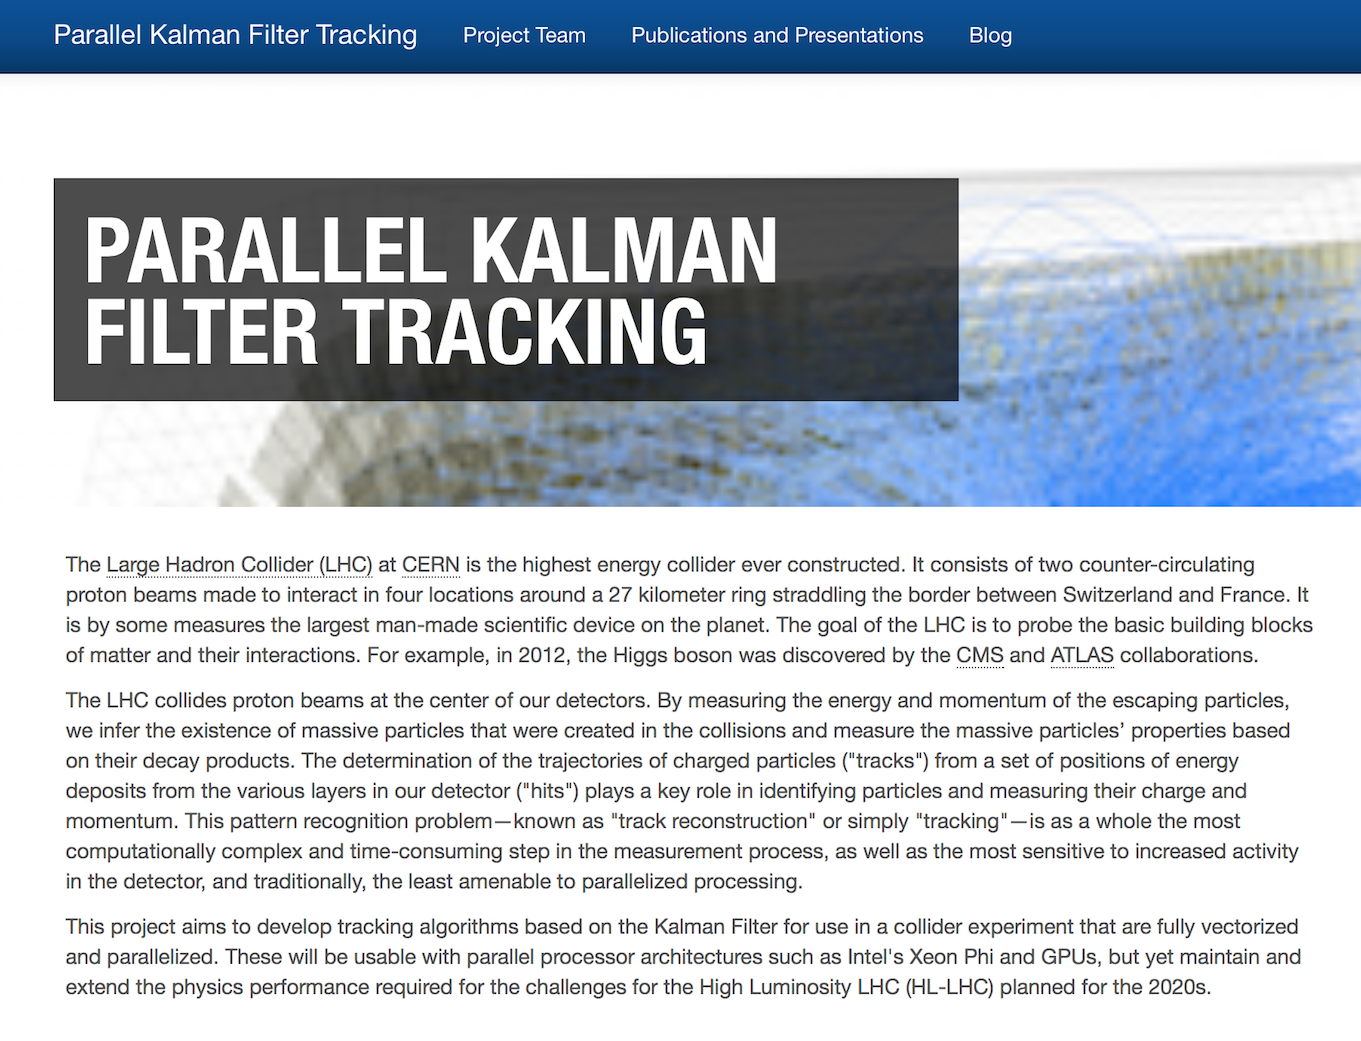
\includegraphics[width=0.7\textwidth]{images/parallel-trackreco.png}
%\caption{}
%\label{fig:example2}
\end{center}
\end{figure}

\small{http://trackreco.github.io}

\end{frame}



\begin{frame}
\frametitle{Summary}

\begin{itemize}
\item There are a number of Software/Computing challenges to prepare for the HL-LHC era: scale, performance/cost, technology evolution and long term sustainability
\item We are working towards a ``software upgrade'' to address these challenges.
\item Over the next year a community roadmap (Community White Paper on Software and Computing, CWP) will be produced with a coherent roadmap for such an upgrade. This will be the basis for efforts to obtain/organize resources.
\item A handful of forward looking projects are underway today. We expect that over the next few years this will grow into the effort required to build the software required for the HL-LHC era in the 2020s.
\end{itemize}



\end{frame}



\begin{frame}
\frametitle{HEP Software Ecosystem}

\begin{figure}[htbp]
\begin{center}
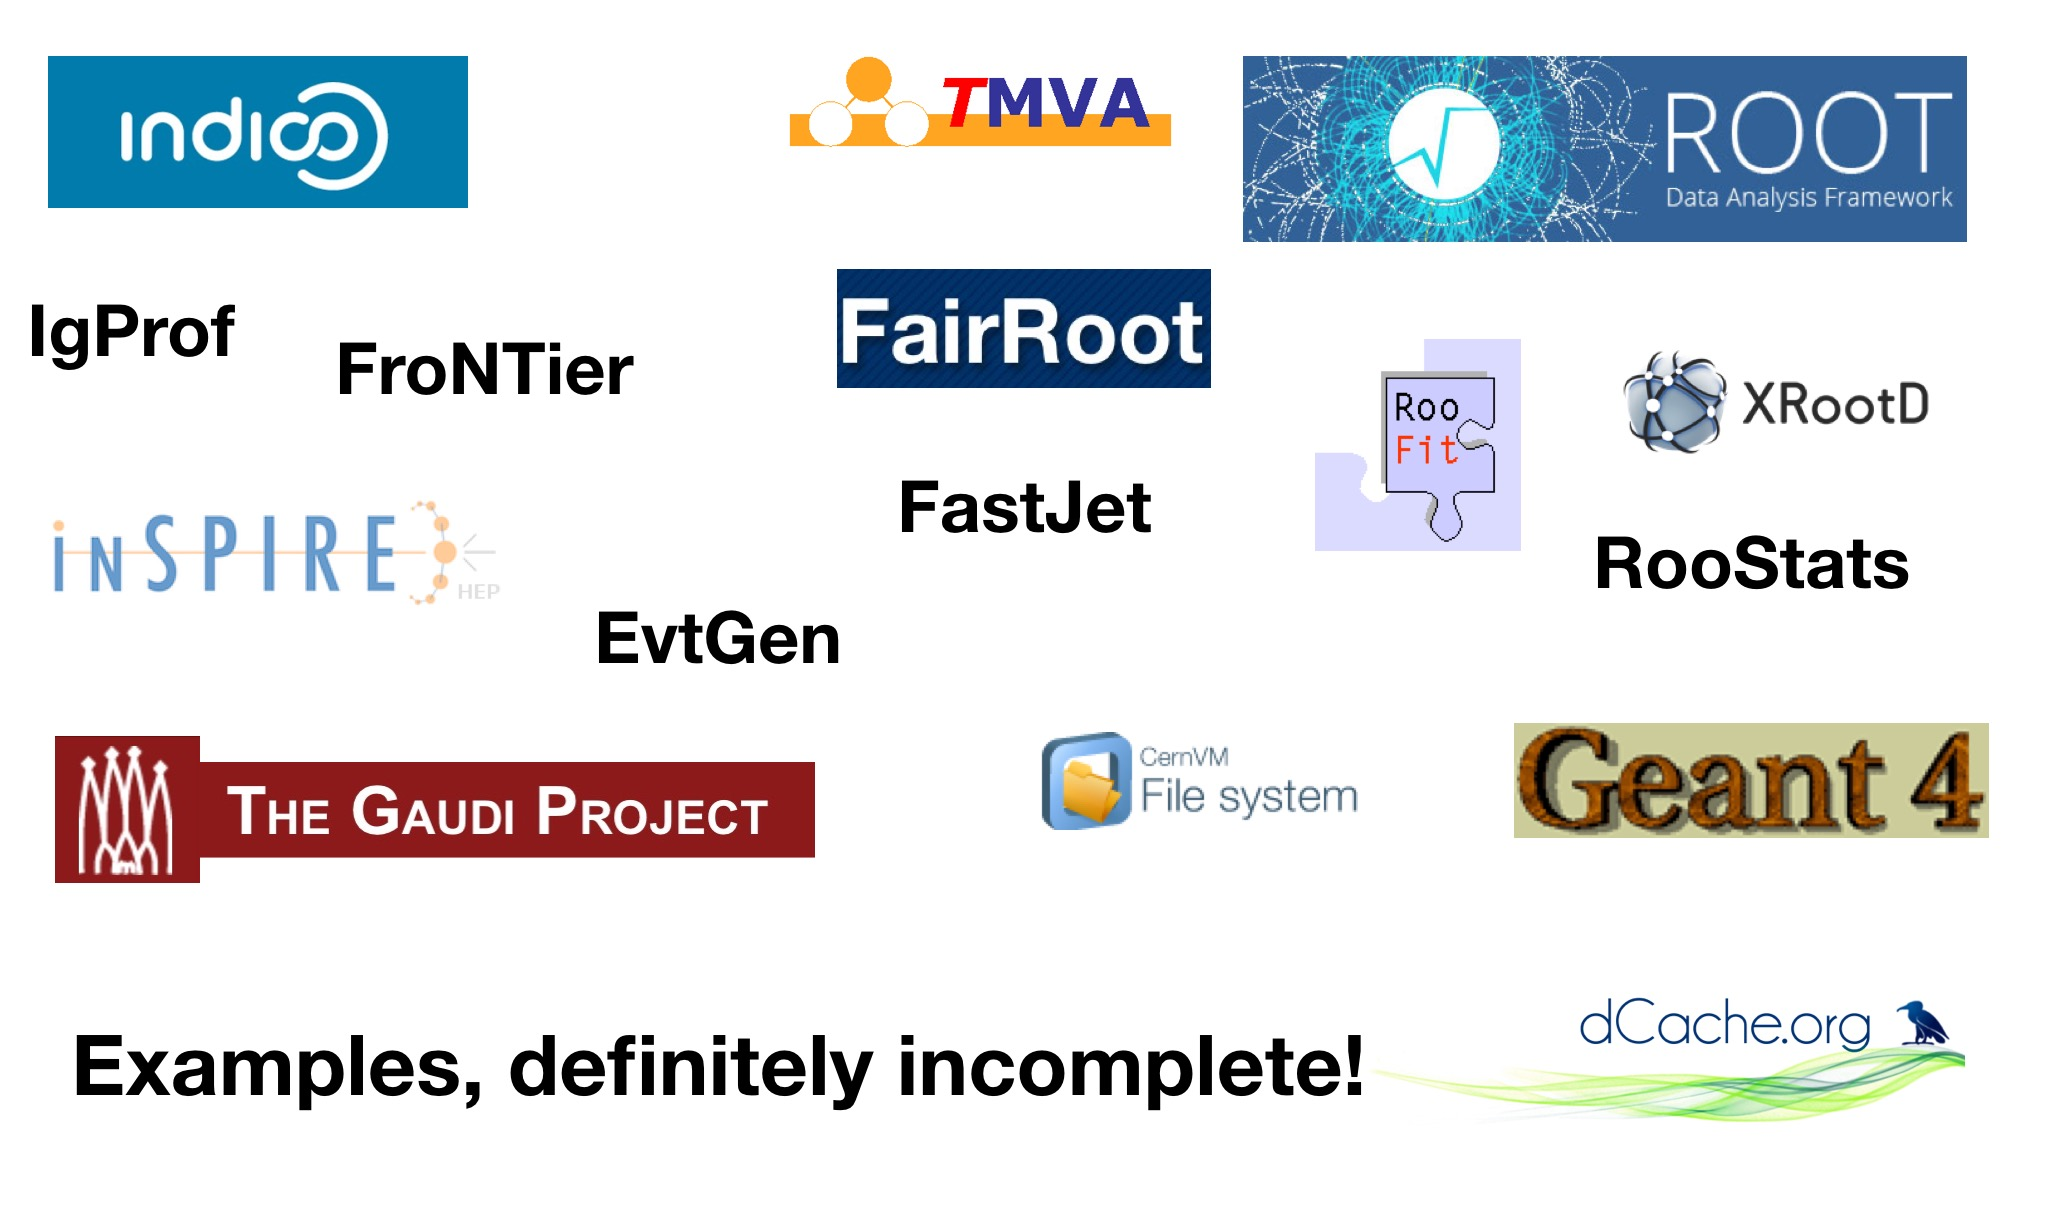
\includegraphics[width=0.9\textwidth]{images/hep-software-ecosystem.jpg}
\end{center}
\end{figure}

\end{frame}




\end{document}


